% 5
\documentclass[output=paper]{LSP/langsci}
\author{Anthony Grant}
%\title{A forgotten figure in Siouan and Caddoan linguistics:  Samuel Stehman Haldeman (1812--1880)}
%\abstract{In the light of Bob Rankin's Dhegiha work this paper examines some of the earliest recorded material on Kanza and Osage, collected and transcribed by the naturalist Samuel Stehman Haldeman in an alphabet of his own devising (\citealt{Haldeman1859; Haldeman1860}).  Although his transcriptions fail to capture many crucial phonetic and phonemic distinctions, they are useful as records of earlier and more conservative  forms of these languages. KEYWORDS: [Kanza, Osage, orthography, phonetic transcription, history of linguistics]}
\title{A forgotten figure in Siouan and Caddoan linguistics:  Samuel Stehman Haldeman (1812-1880)}
\abstract{In the light of Bob Rankin's Dhegiha work this paper examines some of the earliest recorded material on Kanza and Osage, collected and transcribed by the naturalist Samuel Stehman Haldeman in an alphabet of his own devising (\citealt{Haldeman1859,Haldeman1860}).  Although his transcriptions fail to capture many crucial phonetic and phonemic distinctions, they are useful as records of earlier and more conservative  forms of these languages. KEYWORDS: [Kanza, Osage, orthography, phonetic transcription, history of linguistics]}
\ChapterDOI{}

\rohead{A forgotten figure in Siouan and Caddoan linguistics}

\maketitle

\begin{document}

\section{Introduction}

Robert Rankin's examinations of earlier sources on Native American languages which have rarely been the subject of fuller description impel us to look at the work of other early collectors of data on Siouan and Caddoan languages. We may mention for instance his paper on Max von Wied's \citeyearpar{Maximilian18391841} brief vocabulary of Kaw, Kanza or Kansa  (\citealt{Rankin1994}), Nor should we overlook his splendid salvage work on Kanza (the name I will use henceforth in this paper) and Quapaw, and his pivotal role in the organization of the Siouan-Caddoan Conferences.

One researcher is almost overlooked nowadays (despite a memoir by \citealt{Lesley1881} which hymns his activities while getting its dedicatee's name wrong). The naturalist, sawmill manager and avocational linguist Samuel Stehman Haldeman (1812--1880)  was mostly known to the linguists in the 19th century for his `Analytic Orthography' (\citealt{Haldeman1859}, also produced in book form as \citealt{Haldeman1860}). This was a prizewinning attempt to construct a  universal phonetic alphabet, based on Latin letters (and following some precepts of Classical Ciceronian Latin pronunciation, for instance <C> for /k/ and <V> for /w/) but enhanced with some created symbols. It also added a number of diacritics,  for documenting phonetic data in the world's languages, especially from previously undescribed languages of North America and elsewhere.  

This work represented a determined effort to describe and notate speech sounds, for which it was awarded the Trevyllian Prize in London against eighteen contenders. And there its reception ground to a halt. The alphabetic system, based on what Haldeman assumed were Classical Latin letter-values,  was well-adapted to indicate certain aspects of vowel quality and quantity and basic consonantal distinctions. But his pioneering work is one of several such pre-International Phonetic Association  schemes proposed in the 19th century, of which \citet{Lepsius1863} is the most famous and influential, and it is cumbrous.  Because it required a large number of special fonts and diacritics it was difficult to reproduce, with the result that nobody save Haldeman ever adopted it.    

Haldeman's system is elaborate but just how successfully or consistently he applied his own transcriptional system is moot. For instance in his Chinese data (actually Cantonese), he fails to indicate any tones for the numerals for Guangzhou Cantonese, although he makes an effort to do so for  the nearby Macanese variety of Cantonese.  Haldeman uses the phonetic terminology of his time, with \textit{surd, sonant, lenis, asper}, employed where modern phoneticians talk about \textit{voiceless, voiced, unaspirated} and \textit{aspirated} sounds, and with \textit{sigmal, lingual, cerebral, guttural} and \textit{faucal} used for modern \textit{alveolar, dental, retroflex, velar} and \textit{uvular} respectively,    He also talks about ``pure'' (non-nasalized) and  nasal  sounds, and arrays consonants according to their degree of ``interruption'' (plosives are the most ``interrupted'' consonants in this scheme); see \figref{haldemandigest}.   He also divided consonants into \textit{mutes} (plosives and nasals) and \textit{liquids} (other consonants).  \citet[83, 369]{Haldeman1860} recognizes thirty four vowel qualities, which he arranges in a dense A-shaped diagram, and he indicates vowel quantity with macrons and breves.   Unlike Daniel Jones (\citealt{Jones1909}) he does not propose a scheme in which the distinction between back [\textipa{A}] and front [a] is crucial.  

\begin{figure} 
\caption{A digest of consonantal symbols in \citealt[121: \S576]{Haldeman1860}} \label{haldemandigest}
% \begin{rotate}{12} 
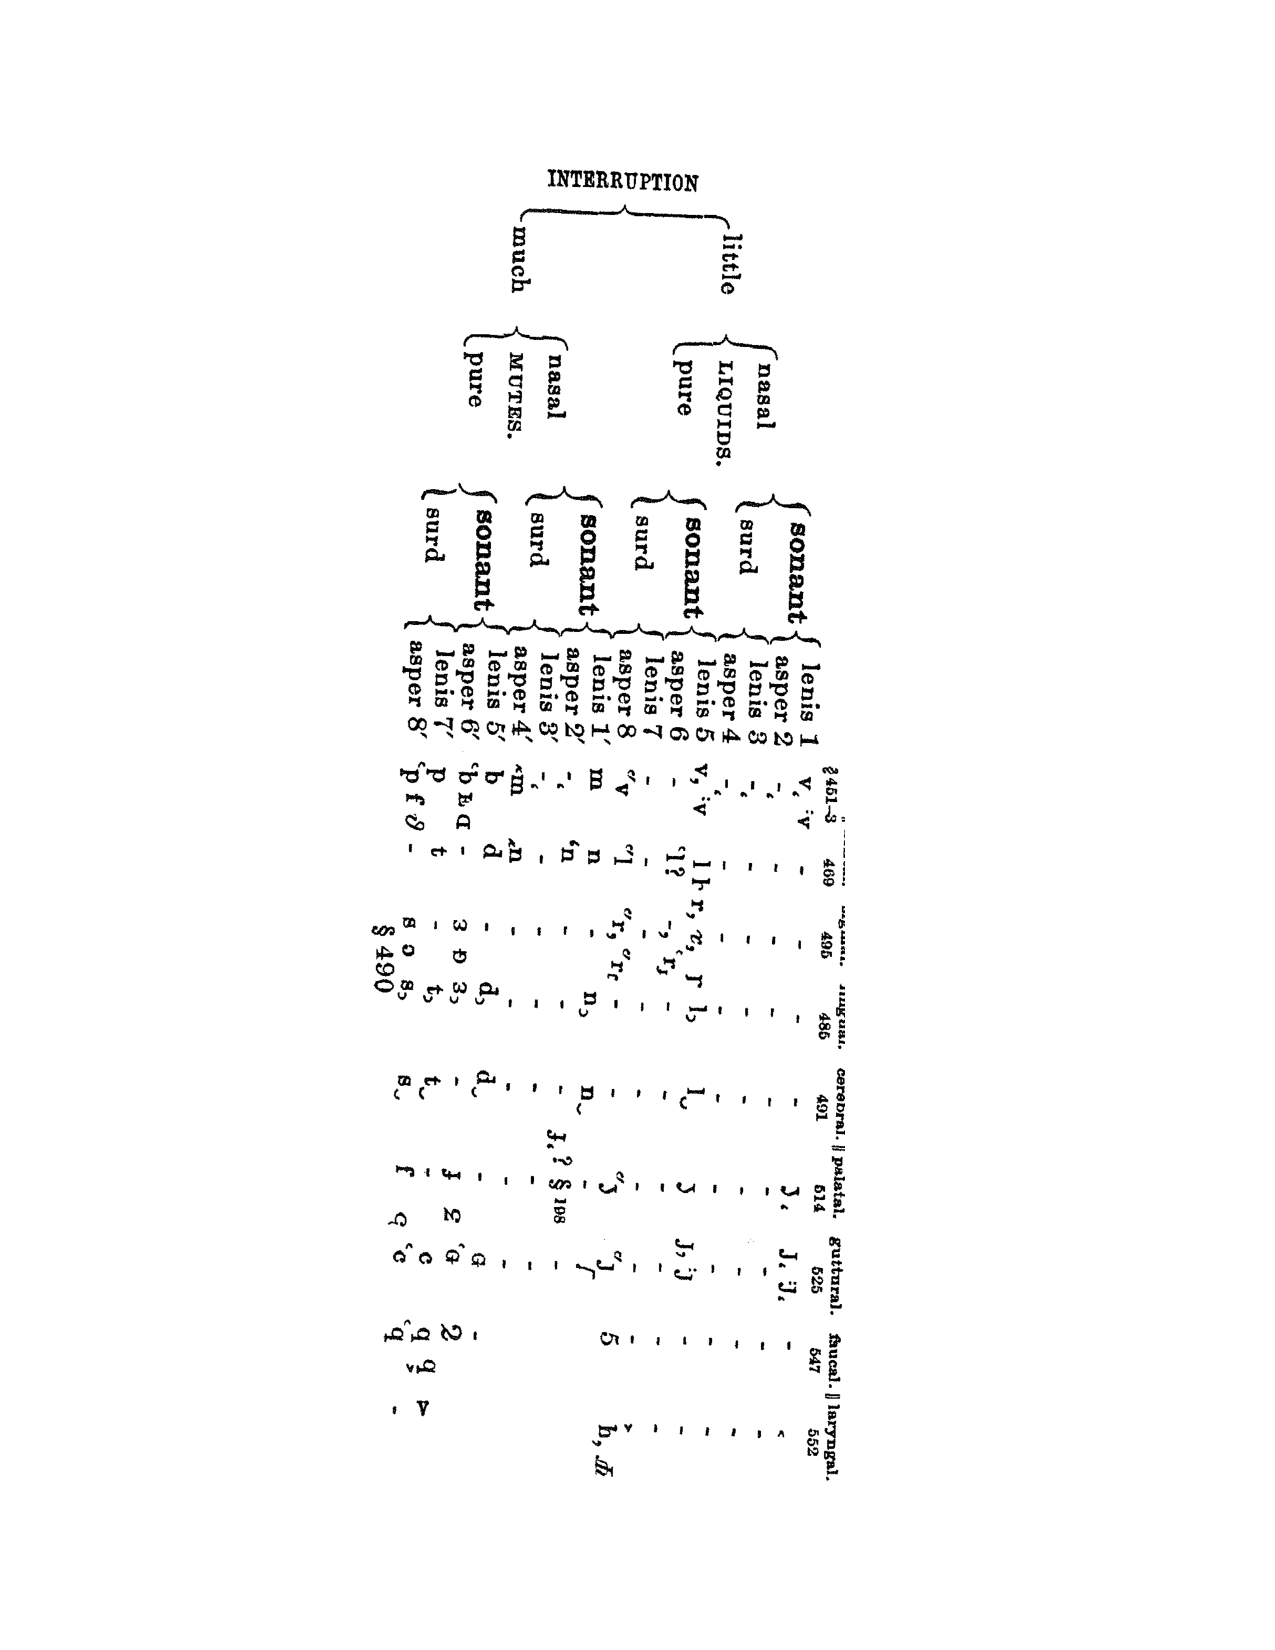
\includegraphics[width=.6\textwidth,angle=92]{figures/GrantConsonants}
% \end{rotate}
\end{figure}

The concentration in this work is on Haldeman's Dhegiha-language data, though observations from his work on Caddo and Wichita will be added where relevant. (Unfortunately I lack sufficient modern lexical data to give as full an analysis with modern examples of the Caddo and Wichita data as I would wish.)   Data from Haldeman's work are taken from \citet{Haldeman1860}, a corrected and book-length edition of \citet{Haldeman1859}.  Haldeman divided his work into sections (often extremely short and usually corresponding to paragraphs), in addition to the book being paginated.  Both modes of reference will be used here.  

\section{Haldeman the Americanist and his work on Dhegiha}  

In addition to a number of versions of the Lord's Prayer (including those in Cherokee and Wyandot) \citet{Haldeman1860}  provided data in the form of 75 cardinal numeral sets from 1--10 from a wide range of languages of Europe, Asia and North America (plus Grebo from Liberia).  A number of these were Algonquian, Muskogean and Iroquoian languages in addition to numerals from Makah, Chinook, Comanche, Jicarilla Apache and the Yuman language Iipay `Aa. Among the languages on which Haldeman tried out his spelling system are the Dhegiha Siouan language Kanza (for which he also provided some Santee parallels for certain forms from \citealt{Riggs1852}; see Figure 3).  He also provided data from the Caddoan languages Caddo (which Haldeman referred to as ``Nadaco'') and Wichita (referred to as ``Waco'' but identical with the Wichita recorded in the 20th and 21st centuries, for instance in \citet{Rood1975}. In each case the data presented are cardinal numerals from 1--10 and some additional lexicon (over 40 such items in the case of Caddo and 10 from Wichita), evidently recorded by Haldeman from native speakers and not previously listed elsewhere. Haldeman also collected the numerals from 1--10 in Osage; see Figures \ref{haldemannumerals} and \ref{haldemanlexicon}.   

\begin{figure}
\centering
\caption{Numeral data from Kanza and Osage (\citealt[3, \S711, 712]{Haldeman1860})} \label{haldemannumerals}
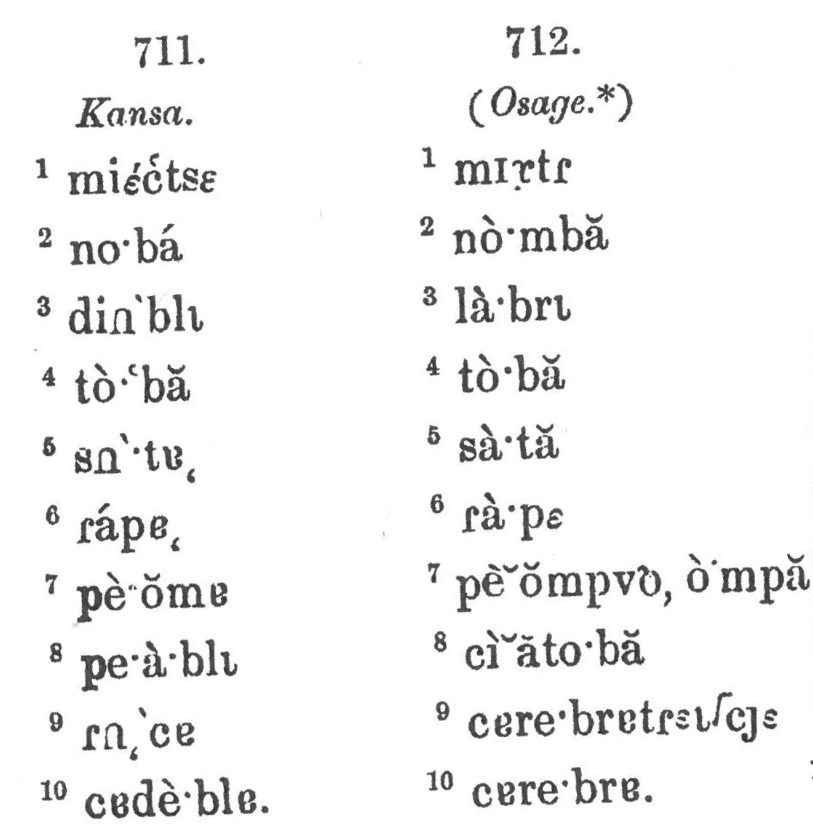
\includegraphics[width=2.5in,angle=-2]{figures/GrantNumerals}
\end{figure}

\begin{figure}
\centering
\caption{Lexicon from Kanza, with some Dakota parallels from \citet{Riggs1852}  (\citealt[3, \S634]{Haldeman1860})} \label{haldemanlexicon}
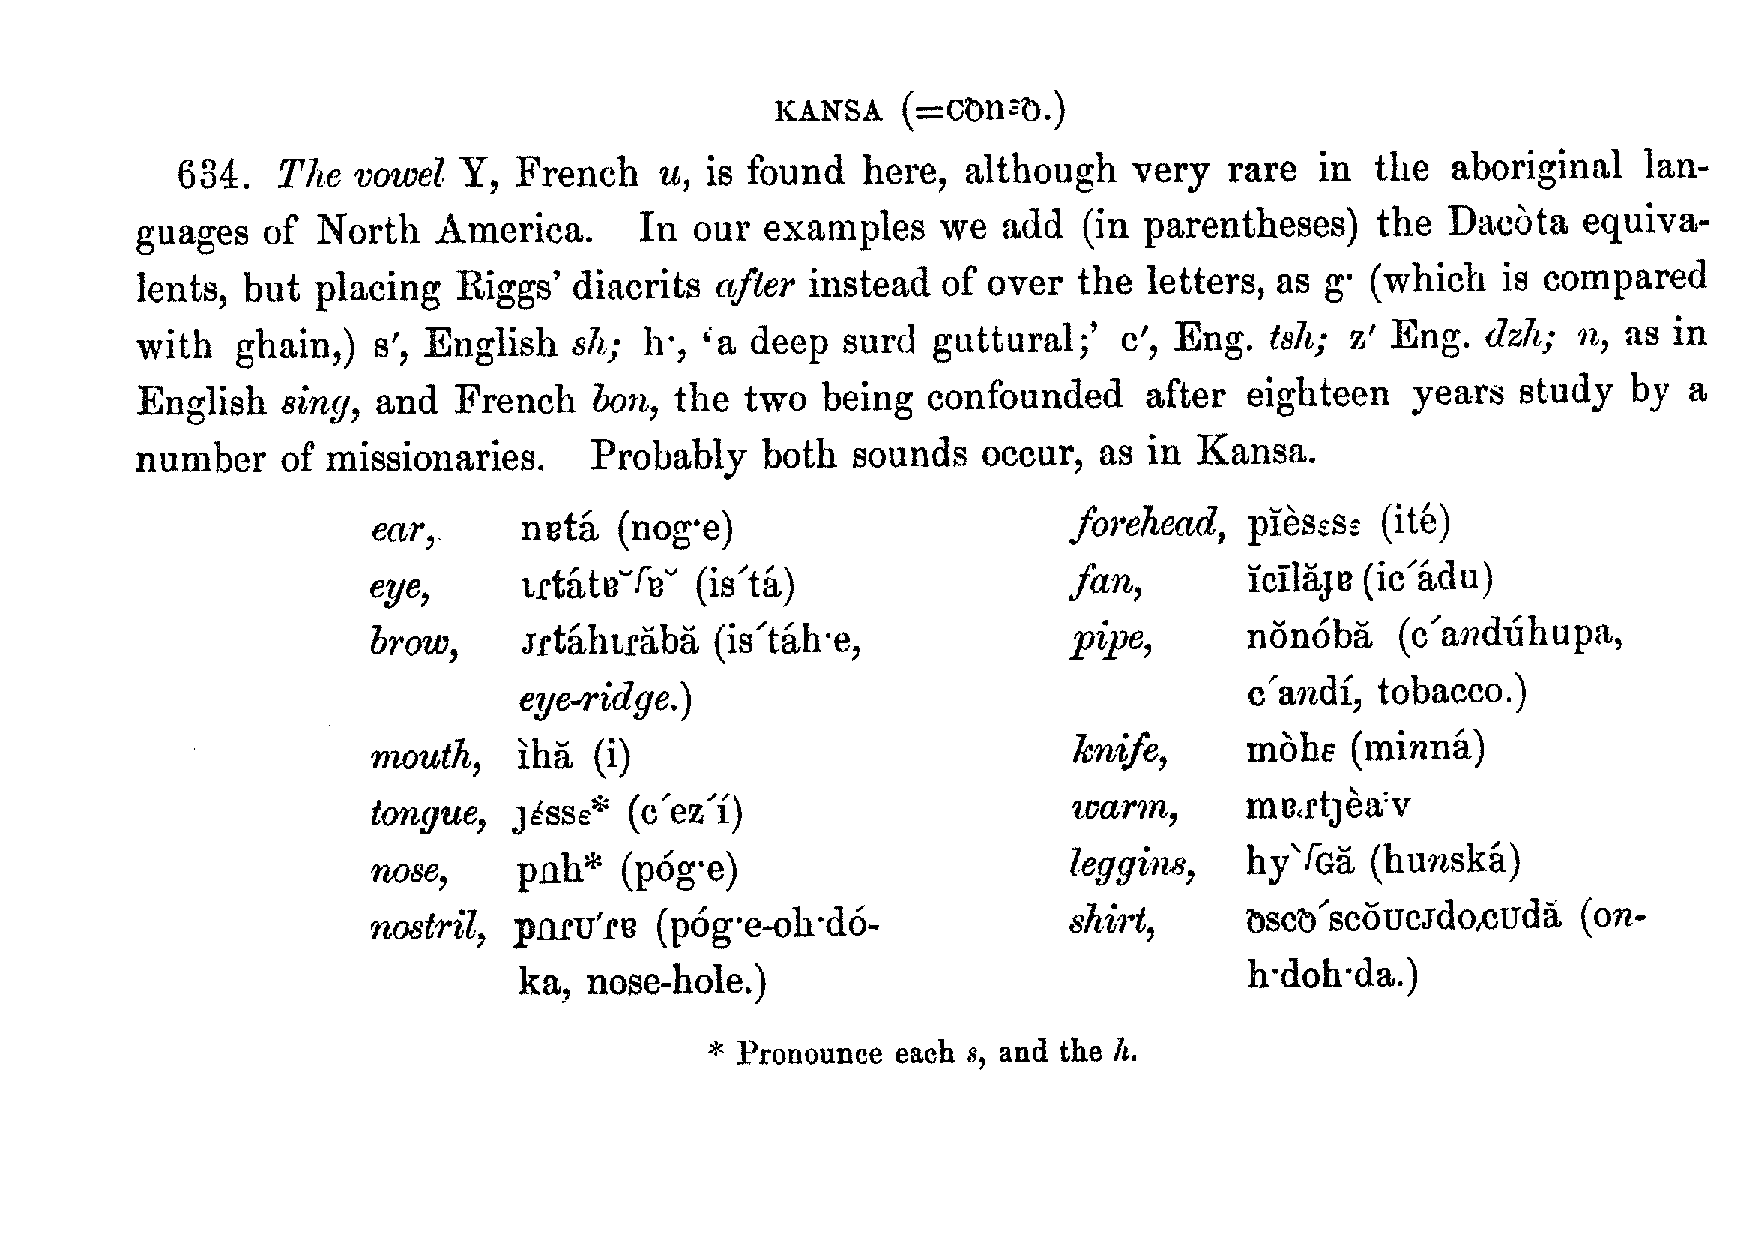
\includegraphics[width=5in]{figures/GrantKanzaWords}
\end{figure}

As \citet{Rankin1994} showed, Max von Wied (\citeyear{Maximilian18391841}) had described sounds in various Dhegiha languages (Wied\ia{Wied, Max von} documented Omaha, Ponca, Kanza and Osage) quite well within the limitations of his annotated Franco-German spelling system. This means that though his work is superb for its time he missed many crucial details and failed to record other details consistently.   Haldeman's system was theoretically more precise as far as it went (although there is little consistent coverage of tones and essentially none of consonants which are ingressive, velaric, or other kinds of clicks). But it was deployed less consistently and less accurately.   His records of Kanza and Osage do show an ability to indicate primary stress using acute accents, while grave accents are used to indicate a variety of vowel qualities, short vowels are marked with breves, long vowels with postvocalic dots, and vowel nasalization is represented with the ogonek or Polish hook placed at the bottom of the line after the vowel.  

Working on small amounts of material (often only the numerals from 1--10) from a large number of languages, Haldeman recognized that some sounds were problematic in terms of his descriptive criteria, as his discussion of the two ejectives  Caddo /t'/ and Wichita /k'/ shows (\citealt[3, \S448; 131, \S574]{Haldeman1860}).  But he did not make the leap (as \citealt{Garcia1760} had done for Coahuilteco) by discovering that what made these sounds distinctive from other speech sounds but similar to one another was their common possession of ejective quality, with the corollary that ejectives should be represented consistently.  As a result he was unable to indicate the ejective quality of the final consonant in Caddo \textit{wists'i} `one'.  In fact, Haldeman's attempts at transcribing Caddo (for instance Haldeman's <v\'{\textipa{A}}t\textipa{5}t'> for \textit{waadat} `earth', in which he fails to hear that the medial stop is voiced: \citealt[3, \S633]{Haldeman1860}) are scattershot enough to be unreliable. Even so he recognized that the Caddo word for `cheek'  used a dental or alveolar rather than a velar nasal.    

His array of consonantal types was defective in other respects. Although Dhegiha languages contain ejectives, the small samples from Kanza and Osage which Haldeman cites happen not to include any of these sounds; Haldeman would probably have been unable to indicate these, as they are not provided for in his consonantal chart, and his encounters with them in Caddo and Wichita left him uncertain as to the nature and phonetic structure of the ejectives which he encountered there.  He also lacked a consistent way of indicating the glottal stop, either initially, medially or finally, which is a special problem when recording Caddo data. Nor did Haldeman's system capture the three degrees of phonemic vowel length which are present in Wichita (although \citealt[3, \S353--355]{Haldeman1860}) provides the wherewithal to do this.  

As a result of these and other shortcomings, Haldeman's work has received rather little attention from modern phonologists or indeed other linguists.  Even Haldeman himself made no use of the system in his work on Pennsylvania German (\citealt{Haldeman1872}).  The discussion in \citet{Pilling1887} and the brief account in \citet{KellyLocal1989}, written incidentally by the academics who taught phonetics to this author, are  rare exceptions to this neglect.   

Haldeman's data on Osage, comprising merely the cardinal numerals from 1 through 10, and the corresponding forms in Kanza, help us to get a better sense of his transcriptional techniques. Modern Osage data are from \citet{Quintero2009} and Kanza data from \citet{CumberlandRankin2012}.  Original transcriptional systems have been preserved. We note that the two languages, though very close, are represented differently in regard to orthographic conventions employed to indicate postalveolar sibilants, vowel length and nasalized vowels. 

Dhegiha languages share a number of crosslinguistically marked features in their segmental phonology.  These include the differentiation of nasalised from oral vowels, the differentiation of geminate and lengthened stops, of preaspirated and voiceless ejective stops, and the use of a high front rounded vowel. Modern forms are given below (Kansa <u> is /y/ and superscript <n> represents nasalization, indicated in Osage by an ogonek).


\section{Modern counterparts of the data}
In Tables \ref{numerals} and \ref{additionallexicon} are given modern equivalents in Kanza and Osage for Haldeman's data in figures 2 and 3. 

\begin{table}
\caption{Cardinal Numerals \citep[\S711, 712]{Haldeman1860}} \label{numerals}
\begin{tabular}{l l l}
\lsptoprule
& Kanza &  Osage \\
\midrule
1 & miⁿxci &  w\k{i}xce  \\
2 & noⁿb\'a  & \textipa{D}\k{o}\k{o}pa  \\
3 & y\'abliⁿ &  \textipa{D}\'aabr\k{i}\k{i} \\
4 & d\'oba	 & t\'oopa \\
5 & s\'ataⁿ	& s\'aht\k{a} \\
6 & sh\'ape & \v{s}\'ahpe \\
7 & p\'eyoⁿba & hp\'ee\textipa{D}\k{o}\k{o}pa \\
8 & kiad\'oba	& hkiet\'oopa \\
9 & sh\'aⁿka & l\'ebr\k{a} hce w\k{i}\k{i}ke \\
10	& gl\'ebla	& l\'ebr\k{a} \\
\lspbottomrule
\end{tabular}
\end{table}

\begin{table}
\caption{Additional Kanza lexicon \citep[\S634]{Haldeman1860}} \label{additionallexicon}
\begin{tabular}{l l}
\lsptoprule
& Kanza \\
\midrule
Ear & naⁿt\'a \\
Eye & isht\'a (note isht\'a toho `iris'  and isht\'akaⁿha  `eyelid') \\
Brow & isht\'ahin \\
Mouth	& i (Haldeman's form iha is `mouth-skin' or `lips') \\
Tongue & l\'eze \\
Nose & pa \\
Nostril	& pa xl\'oge \\
Forehead	& pe \\
Fan & ij\'eayuz\'ube (fan hung over baby's face) \\
Pipe & nann\'onba \\
Knife & m\'anh\'in \\
Warm	& moshc\'e \\
Leggins [sic] & h\'uyuyinge \\
Shirt & \'okiloxla \\
\lspbottomrule
\end{tabular}
\end{table}

 Note that what are written as single plosives in the modern Kanza orthography are actually geminates, thus <k> is /kk/.  

\section{Remarks on the forms}
The materials here represent examples of impressionistic phonetic transcriptions, which is what we would expect in a work from the pre-phonemic era.  The Kanza and Osage words in Haldeman's material (especially the former) are recorded with comparatively greater detail than numerical data from some of the other languages are.  Indeed the Kanza numerals are recorded with greater detail by Haldeman with respect to accent than they are in the present orthography.  But the forms are not necessarily noted with greater accuracy, and neither system indicates the differences between the various voiceless stop series clearly.   Tense stops in Kanza in Haldeman's transcription are represented by the use of bold consonantal characters, so that  Haldeman's <p> is [p $\sim$ ph], <\textbf{p}> is [pp] while <`p> is [hp] in his Kanza work. (This fact is clearer in the version of Haldeman's work published in the Transactions of the American Philosophical Society than in the acid-heavy and aged brown paper of the version of \citealt{Haldeman1860} available from archive.org).  

The forms are in general readily identifiable from recording of the languages over a century later, as the references from the Kanza and Osage dictionaries show (\citealt{CumberlandRankin2012} for Kanza, and \citealt{Quintero2009} for Osage). The few differences are instructive.    

Most interesting in this regard are the numerals, especially `nine' and `ten'.  In Osage `nine' is a subtractive compound (`ten lacking one') involving `ten' and an allomorph of `one'.  But  Kanza uses the widespread form, possibly reconstructible as \textit{ki\v{s}\k{a}kka}, which is recorded for several Mississippi Valley and Ohio Valley Siouan, Muskogean and Great Lakes Algonquian languages.   Modern Osage has simplified the onset of `ten', though Haldeman had what would nowadays be represented as /kar-/ (or maybe /gar-/; his depiction of voicing is not always trustworthy).  The form in Dhegiha has irregular reflexes elsewhere in Dhegiha:   Omaha-Ponca \textit{gth\'eba},\footnote{\url{http://omahalanguage.unl.edu/dictionary/}} where <th> is /\textipa{D}/, has lost the liquid found in the second syllable in other Dhegiha languages and in earlier records of Omaha-Ponca (compare Quapaw \textit{kd\'ebn\k{a}}: \citealt[3]{Rankin1982}). The glide which separates the prefix from the form for `three' in Kanza `eight' has been apprehended by Haldeman as a front vowel, although the hiatus in the corresponding Osage form has been recognized by Haldeman as such.  

Both the Kanza and Osage forms in Haldeman's work include forms of what was originally the enclitic \textit{-xci} `only' at the end of the form for ONE, and this pan-Dhegiha word is a form which was later borrowed into Caddo as \textit{wists'i'}.  Note also the initial [di-] in Kanza `three', now replaced by /j-/ <y->, and the fact that Haldeman did not notice the nasalization of the vowel in the first syllable of Kanza `two'.  The form `eight' in Haldeman's Osage is reflected in the modern language, in modern Kanza and (as a loan, namely \textit{kiy\'ataw}: \citealt{Rood1996}:608) in modern Wichita. But the earlier form for `eight' based on `three' is used in Haldeman's Kanza as a parallel to the form for `seven' (itself a compound involving `two'). Primary stress and vowel length and nasalization are well represented in Haldeman's work, especially for Osage.  

Of the nouns in Haldeman's record of Kanza, most are similar to their modern counterparts.  For the rest, if one allows for a modicum of close phonetic detail (for instance the realization of /a/ as a low rounded vowel in `nose'), the quality of transcription is rather high. `Eyebrow' may end in a form of \textit{s\'abe} `black' but this is uncertain, while material which is less easy to identify is attached to the end of `eye' and `shirt'.  The occasional weakness in Haldeman's powers of perception is seen in the fact that the consonantal sounds in the second part of `nostril' are represented in Haldeman's work by his symbol for /\textipa{S}/, while the initial consonant of `tongue' has changed in the 120 or so years between Haldeman's work and Bob Rankin's.  `Warm' seems to include an enclitic, which may be the masculine declarative enclitic \textit{(ey)ao}.  Haldeman's remarks about the phonetics of `nose' and `tongue' are somewhat surprising, as modern Kanza does not permit [h] in coda position and does not use geminate consonants.


\section{Conclusion}
Data on Haldeman's recording of Dhegiha language data have been presented and the success or otherwise of Haldeman's system in coping with the segmental phonology of these languages, especially the complex consonantal systems, has been evaluated. Haldeman's ability correctly to hear the phonetic features of a language seems to have varied in competence from one language to another.  Although his Kanza and Osage data are the most accurately recorded Dhegiha data of their time (and although very little else was available for Kanza when Haldeman's data appeared), his transcription is still far from adequate.  This is possibly the result of his imperception of certain sounds.  Nonetheless the transcriptions list some forms which differ in phonological shape or sense from the modern forms of these words, and as such they have some historical significance. 

\section*{Acknowledgment}
I first heard of Bob's\ia{Rankin, Robert L.} Siouan work in the 1980s and grew to know it better in the course of the following decade, thanks to his generosity and that of Dave Costa\ia{Costa, David}, which I eagerly acknowledge. Bob's example of someone switching linguistic fields and taking the opportunity to document languages before they passed completely out of existence (which he accomplished at a time before language endangerment was regarded as an important concern) impressed me greatly, as did his use of philological sources. Having presented a paper at the Siouan-Caddoan Conference I was lucky enough to have dinner with him and Giulia Oliverio\ia{Oliverio, Giulia} at the SSILA Meeting in Albuquerque in 1995, where he was kindly, erudite and hilarious company. The study of Native American language is so much the poorer for his passing.

\printbibliography[heading=subbibliography,notkeyword=this]

\end{document}
